\chapter{Theoretical Foundations}
In this chapter, the theoretical Foundations of deep learning model will be introduced. 
\section{Basis of deep learning}
\subsection{Basic concept}
    In \cite{Goodfellow-et-al-2016}, the concept of deep learning is well described. The deep learning is actually a solution that allows 
    computer to learn from the experiences and understand the world. The entire world consists of hierarchical concepts and relations between 
    each concept with the simpler concept in the next level are also included. This concept of structural hierarchy allows computers to learn 
    from some simple concepts to deeper concepts to solve complex problems, see \autoref{Computer learns from the hierarchical structure of concepts}.
    \begin{figure}
		\centering
		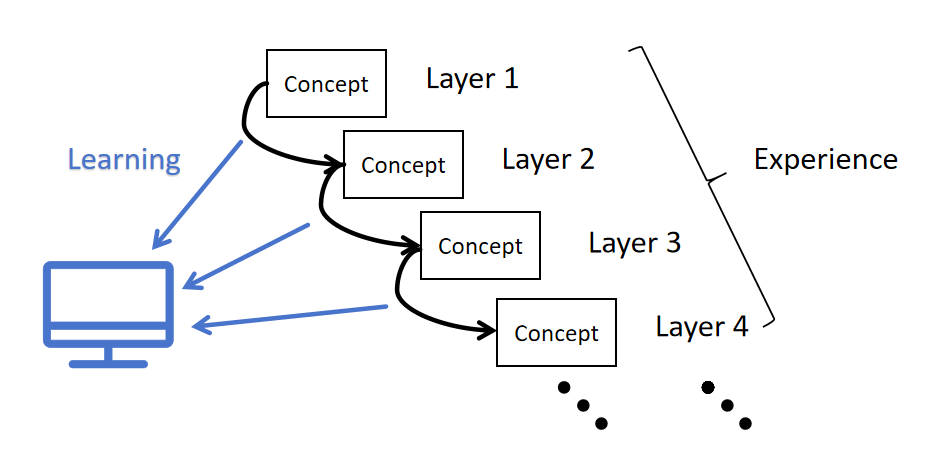
\includegraphics[width=0.9\linewidth]{example_images/ConceptDL}
		\caption{Computer learns from the hierarchical structure of concepts}
		\label{Computer learns from the hierarchical structure of concepts}
	  \end{figure}
    The more layers the structure has, the deeper concepts the computer can learn. After the learning, computers can predict phenomenon and make decisions 
    based on what they have learned. The high-level schematic could be summarized in \autoref{The high-level schematic of deep learning}. The phenomenon or object 
    of interests is the input of the deep learning model. Some simple features will be extracted through sensors, for example the image of the wire harness is extracted 
    through RGB-Camera. The following deep neural network(DNN) can extract more abstract features from the simple features and the computer learns the relations between 
    the features after different layers. After the DNN, the further extracted abstract features should be mapped to the output.  
    \begin{figure}
      \centering
      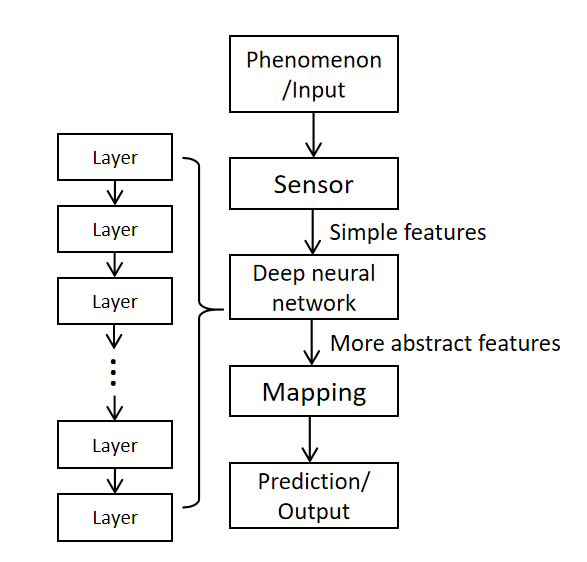
\includegraphics[width=0.6\linewidth]{example_images/DeepLearningSchematic}
      \caption{The high-level schematic of deep learning}
      \label{The high-level schematic of deep learning}
    \end{figure}
  \subsection{Dense neural networks}
  The basic principles of how deep learning works were clarified in the previous section. The next questions are: what is the layer? How does it work to extract features?\\
  In order to answer these two questions more intuitively, the simplest neural network architecture, Dense Neural Network (DNN)\cite{inproceedings}, should be introduced firstly. 
  The DNN simulates the activities of the human brain, which is composed of multiple layers. There could be many neurons in each layer, and all of them are fully connected to 
  all the neurons in the previous layer, see \autoref{Dense neural network}
  The input of the first dense layer is defined as $x_{0}$ and it is also the simple input feature of the network. And the next extracted abstract features are defined as $x_{l}$, 
  where l presents the level of the layer, see \autoref{Mathematical explanation of the feature extraction by layers}.
  The layers are actually defined as some first-order linear mathematical expressions $L _{l}$ with the nonlinear activation function $\Phi_{l}$ in \autoref{eq:layer}, 
  where $w$ is the weight and $b$ is the bias. The nonlinear activation function is important. Without it, the output could be just represented from input by one single layer linearly,
  which is not enough to learn the most of the concepts in the world. Some activation functions are explained in \cite{0706bf17a845490688ef4d7d19df65ba}, e.g., ReLU in \autoref{eq:ReLU}, 
  Sigmoid in \autoref{eq:Sigmoid}, Softmax in \autoref{eq:softmax}. The final step of Schematic, Mapping, can actually be regarded as a layer, which has different options depending on 
  the specific task. For example, for classification, the output layer could be softmax, because it maps the features to probabilities. 
  \begin{figure}
    \centering
    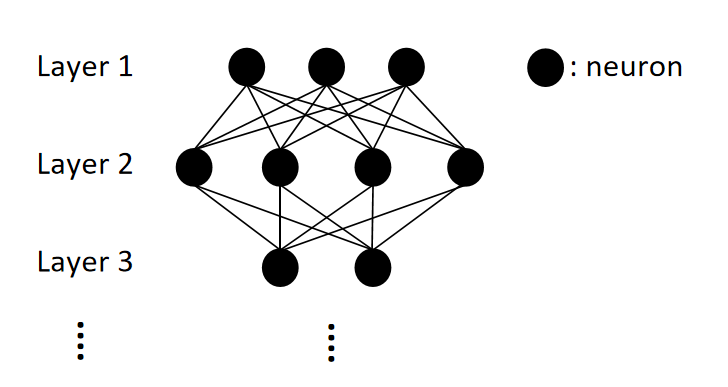
\includegraphics[width=0.6\linewidth]{example_images/DNN}
    \caption{Dense neural network}
    \label{Dense neural network}
  \end{figure}
  \begin{figure}
    \centering
    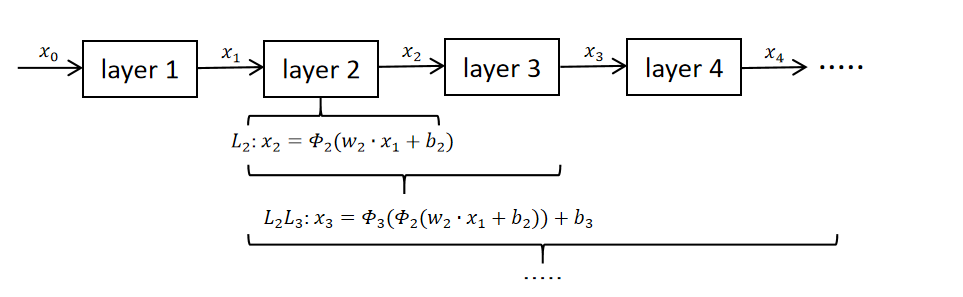
\includegraphics[width=0.9\linewidth]{example_images/mathLayers}
    \caption{Mathematical explanation of the feature extraction by layers}
    \label{Mathematical explanation of the feature extraction by layers}
  \end{figure}
  \begin{align}
    x_{l}=\Phi _{l}(w_{l} \cdot x_{l-1}+ b_{l-1})
     \label{eq:layer}
  \end{align}

  \begin{align}
    \Phi(x) = \begin{cases}
      x& \text{ if } x\ge 0 \\
      0& \text{ else } 
    \end{cases}
     \label{eq:ReLU}
  \end{align}

  \begin{align}
    \Phi(x) = \frac{1}{1+exp(x)^{-1}}  
     \label{eq:Sigmoid}
  \end{align}

  \begin{align}
    \Phi(x_{i}) = \frac{exp(x_{i})}{\sum_{j}exp(x_{j}) } 
     \label{eq:softmax}
  \end{align}
  \subsection{Optimization through backpropagation}
  So far, the process of how initial simple features are extracted and transformed step by step into deeper features through different layers and finally mapped into outputs, 
  i.e., predictions, has been well explained. Then a further question follows: how do networks make accurate predictions?\\
  The transformations and mapping are basically performed by \autoref{eq:layer}. Its result is determined by the activation function $\Phi$, weights $w$ and bias $b$. 
  A GroundTruth $y^{\star }$ needs to be artificially introduced to guide the network to learn the correct behavior, i.e. to predict the desired output. This is explained as
  learning from examples in \cite{russel2010}, which is also well-known as supervised learning. \\
  The prediction of the model or the output after mapping is defined as $y$. A Loss function could be derived. y is actually the result of Mapping, which is actually the output 
  of activation function $\Phi(x)$. It can be further backpropagated onto the feutures from last layer. The optimal weight $w^{star}$ and bais $b^{star}$ are obtained by 
  minimizing the loss equation, see \autoref{eq:Optimization by loss function}. 
  \begin{align}
    w_{l-1}^{\star}, b_{l-1}^{\star}=arg\min_{w_{l-1},b_{l-1}}(\Phi_{l}(\Phi_{l-1}(w_{l-1}\cdot x_{l-1}+b_{l-1}))-y^{\star } ) 
     \label{eq:Optimization by loss function}
  \end{align}
  This approach of optimization can be backwards until the weights and bias of all Layers in the network have been optimized and updated. The whole process is illustrated in 
  \autoref{Parameters are optimized by backpropagation}.
  \begin{figure}
    \centering
    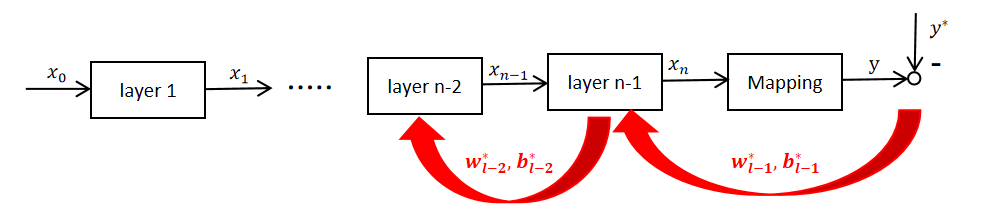
\includegraphics[width=0.9\linewidth]{example_images/bachpropagation}
    \caption{Parameters are optimized by backpropagation}
    \label{Parameters are optimized by backpropagation}
  \end{figure}
  \subsection{Loss Function}
  The loss function in deep learning describes the difference between the groundtruth and the predicted output. The model parameters are optimized and updated by minimizing 
  this function and backpropagating. The loss function could be minimized because it has a gradient $G$. In \autoref{The loss decreases along the direction of the gradient},
  $\theta$ is the model parameter, such as weight, bias. If the gradient is so small, then the loss is difficult to converge. Or if it is so big, then the loss changes oscillatory.
  Hence, a proper loss function is important for deep learning. 
  \begin{figure}
    \centering
    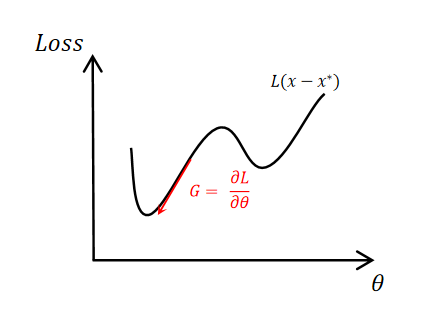
\includegraphics[width=0.6\linewidth]{example_images/loss function}
    \caption{The loss decreases along the direction of the gradient $G$}
    \label{The loss decreases along the direction of the gradient}
  \end{figure}
  For example, l1 in \autoref{eq:l1 loss} and l2-loss function in \autoref{eq:l2 loss} are widely used for regression tasks.
  \begin{align}
    l_1=\sum_{i=1}^{n} \left | y-y^{\star} \right |  
     \label{eq:l1 loss}
  \end{align}
  \begin{align}
    l_2=\sum_{i=1}^{n}(y-y^{\star})^2
     \label{eq:l2 loss}
  \end{align}
  In contrast to the l1-loss function, which is not differentiable at zero, l2 is more often chosen as the loss function because the l2 loss equation is differentiable everywhere.
  But there is also a drawback of l2-loss. When there is an unusual data, the l2 loss will become huge due to squaring. It will affect the training. So the choice of loss function 
  needs to be considered depending on different situations, and sometimes it is necessary to test the effect of different loss functions by doing experiments. In \cite{Sun_2018_ECCV},
  they experimented both l1 and l2-loss for the joint regression task and found that l1-loss function worked consistently better than l2-loss function.\\
  Some other loss functions for segmentation tasks are also introduced in \cite{azad2023loss}. Cross Entropy(CE) loss, in \autoref{eq:CE loss}, is used to the difference between two
  probability distributions. $y^{\star}$ is a one-hot encoded vector and only the targets will be considered.
  \begin{align}
    L_{CE}(y,t) = -\sum_{i=1}^{n} y^{\star} \cdot log(y_{i})
     \label{eq:CE loss}
  \end{align}
  \subsection{Hyperparameter}
  In contrast to the model parameters, hyperparameters cannot be optimized at the backpropagation, but they affect the performance of the model in the meantime as well. 
  In \cite{4e568dfccc734aa6a8184f781bac6353}, the hyperparameters are divided into two groups: (1) performance-oriented parameters, which could influence the system's processing
  throughout, such as the number of threads working simultaneously, i.e., number of workers. (2) accuracy-oriented parameters, which could influence the accuracy of the training, e.g.,
  learning rate and drop out probabilities. There is an overlap between these two groups, and some parameters will affect them both, such as the batch size.\\
  Proper hyperparameters are very important for the training, which significantly affects the accuracy and system performance of the model. And tuning hyperparameters requires experience 
  and patience from researchers, because there might be trade-off between some parameters, for example in \autoref{Trade-off between batch size}, When the batch size increases, the 
  accuracy of the model increases and the system performance decreases.
  \begin{figure}
    \centering
    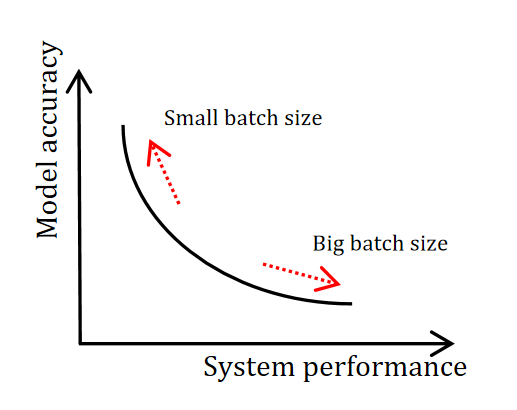
\includegraphics[width=0.6\linewidth]{example_images/batchSize}
    \caption{Trade-off between batch size}
    \label{Trade-off between batch size}
  \end{figure}
\section{Convolutional neural network}
  DNN can extract very deep features by connecting multiple layers. But Yann LeCun in \cite{LeCun1995-LECCNF} also pointed out some drawbacks:
  \begin{itemize}
    \item [1)] The number of parameters is huge and grows quadratically with the number of neurons per layer, which could lead to the problems like overfitting and memories.
    \item [2)] The topology of the input is entirely ignored and it is not suitable to learn global features due to the full connections of neurons. But the image 
    has a strong 2D local structure. Therefore, images are also not suitable as inputs to DNN.
  \end{itemize}
  Convolutional neural network(CNN) doesn't suffer from either of these problems because of the  weight sharing technique and local connectivity. 
  The input is defined as a 2D-image with $C_{l-1}$ channels, length $H_{l-1}$ and width $W_{l-1}$. The convolutional layer is a four dimensional tensor $C_{l-1} \times C_{l} \times K_{l} \times K_{l}$,
  which means it has $C_{l}$ kernels and each kernel has $C_{l-1}$ filters of size $K_{l} \times K_{l}$. Each channel of the input corresponds to a filter of the kernel. All channels corresponding to 
  the sliding window are mapped into a new channel for the output through all filters of a kernel, see \autoref{Convolutional neural network}. The relationship between the size of the output and 
  the size of the input is shown in \autoref{eq:CNN size change}. When extract the deep features of images, the size of the image will be compressed and the number of channels will increase.
  \begin{figure}
    \centering
    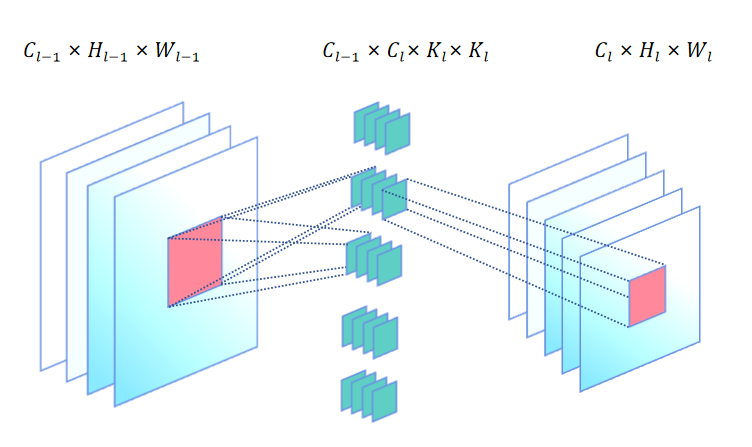
\includegraphics[width=0.9\linewidth]{example_images/CNN}
    \caption{Convolutional neural network}
    \label{Convolutional neural network}
  \end{figure}
  \begin{equation}
  \begin{aligned}
    H_{l}&=H_{l-1}-K_{l}+1\\
    B_{l}&=B_{l-1}-K_{l}+1
      \label{eq:CNN size change}
  \end{aligned}
  \end{equation}
  It is also possible to add modifications to the convolution, such as padding $P$, stride $S$, dialation $D$. When all modifications are included, the size of output image is in \autoref{eq:Modifications} 
  \begin{equation}
  \begin{aligned}
    H_{l}&=\frac{H_{l-1}+2P-(k_{l}-1)D-1}{S}\\
    W_{l}&=\frac{W_{l-1}+2P-(k_{l}-1)D-1}{S}
      \label{eq:Modifications}
  \end{aligned}
  \end{equation}
\section{Transformer}
  In this section, the transformer will be introduced in detail. Think about keypoint detection tasks for the wire harness. The background is regarded as 
  the disturbance. The basic idea is ignoring the non-relevant part and only focusing on the wire harness. 
  The original model architecture of the transformer is shown in \autoref{The Transformer model architecture}. It consists an encoder and decoder structure. 
  It was initially employed to process natural language processing (NLP) tasks such as text translation and generation. The input is defined as three parts:
  query(Q), key(K) and value(V). The query can be viewed as the vector form of a word in text. It could correspond to several keys, which represent vectors of the all words 
  in a text. The value represents the extracted information vector from the all words. $Attention(Q, K)$ represents the match between the query and the corresponding keys 
  and is usually calculated in \autoref{eq:Calculate attention}, where $d_k$ is the dimension of the key vector for avoiding a too large numerator.
  \begin{equation}
    \begin{aligned}
      Attention(Q,K)=\frac{Q\cdot K^T}{\sqrt{d_{k}}} 
        \label{eq:Calculate attention}
    \end{aligned}
    \end{equation}
  \begin{figure}
    \centering
    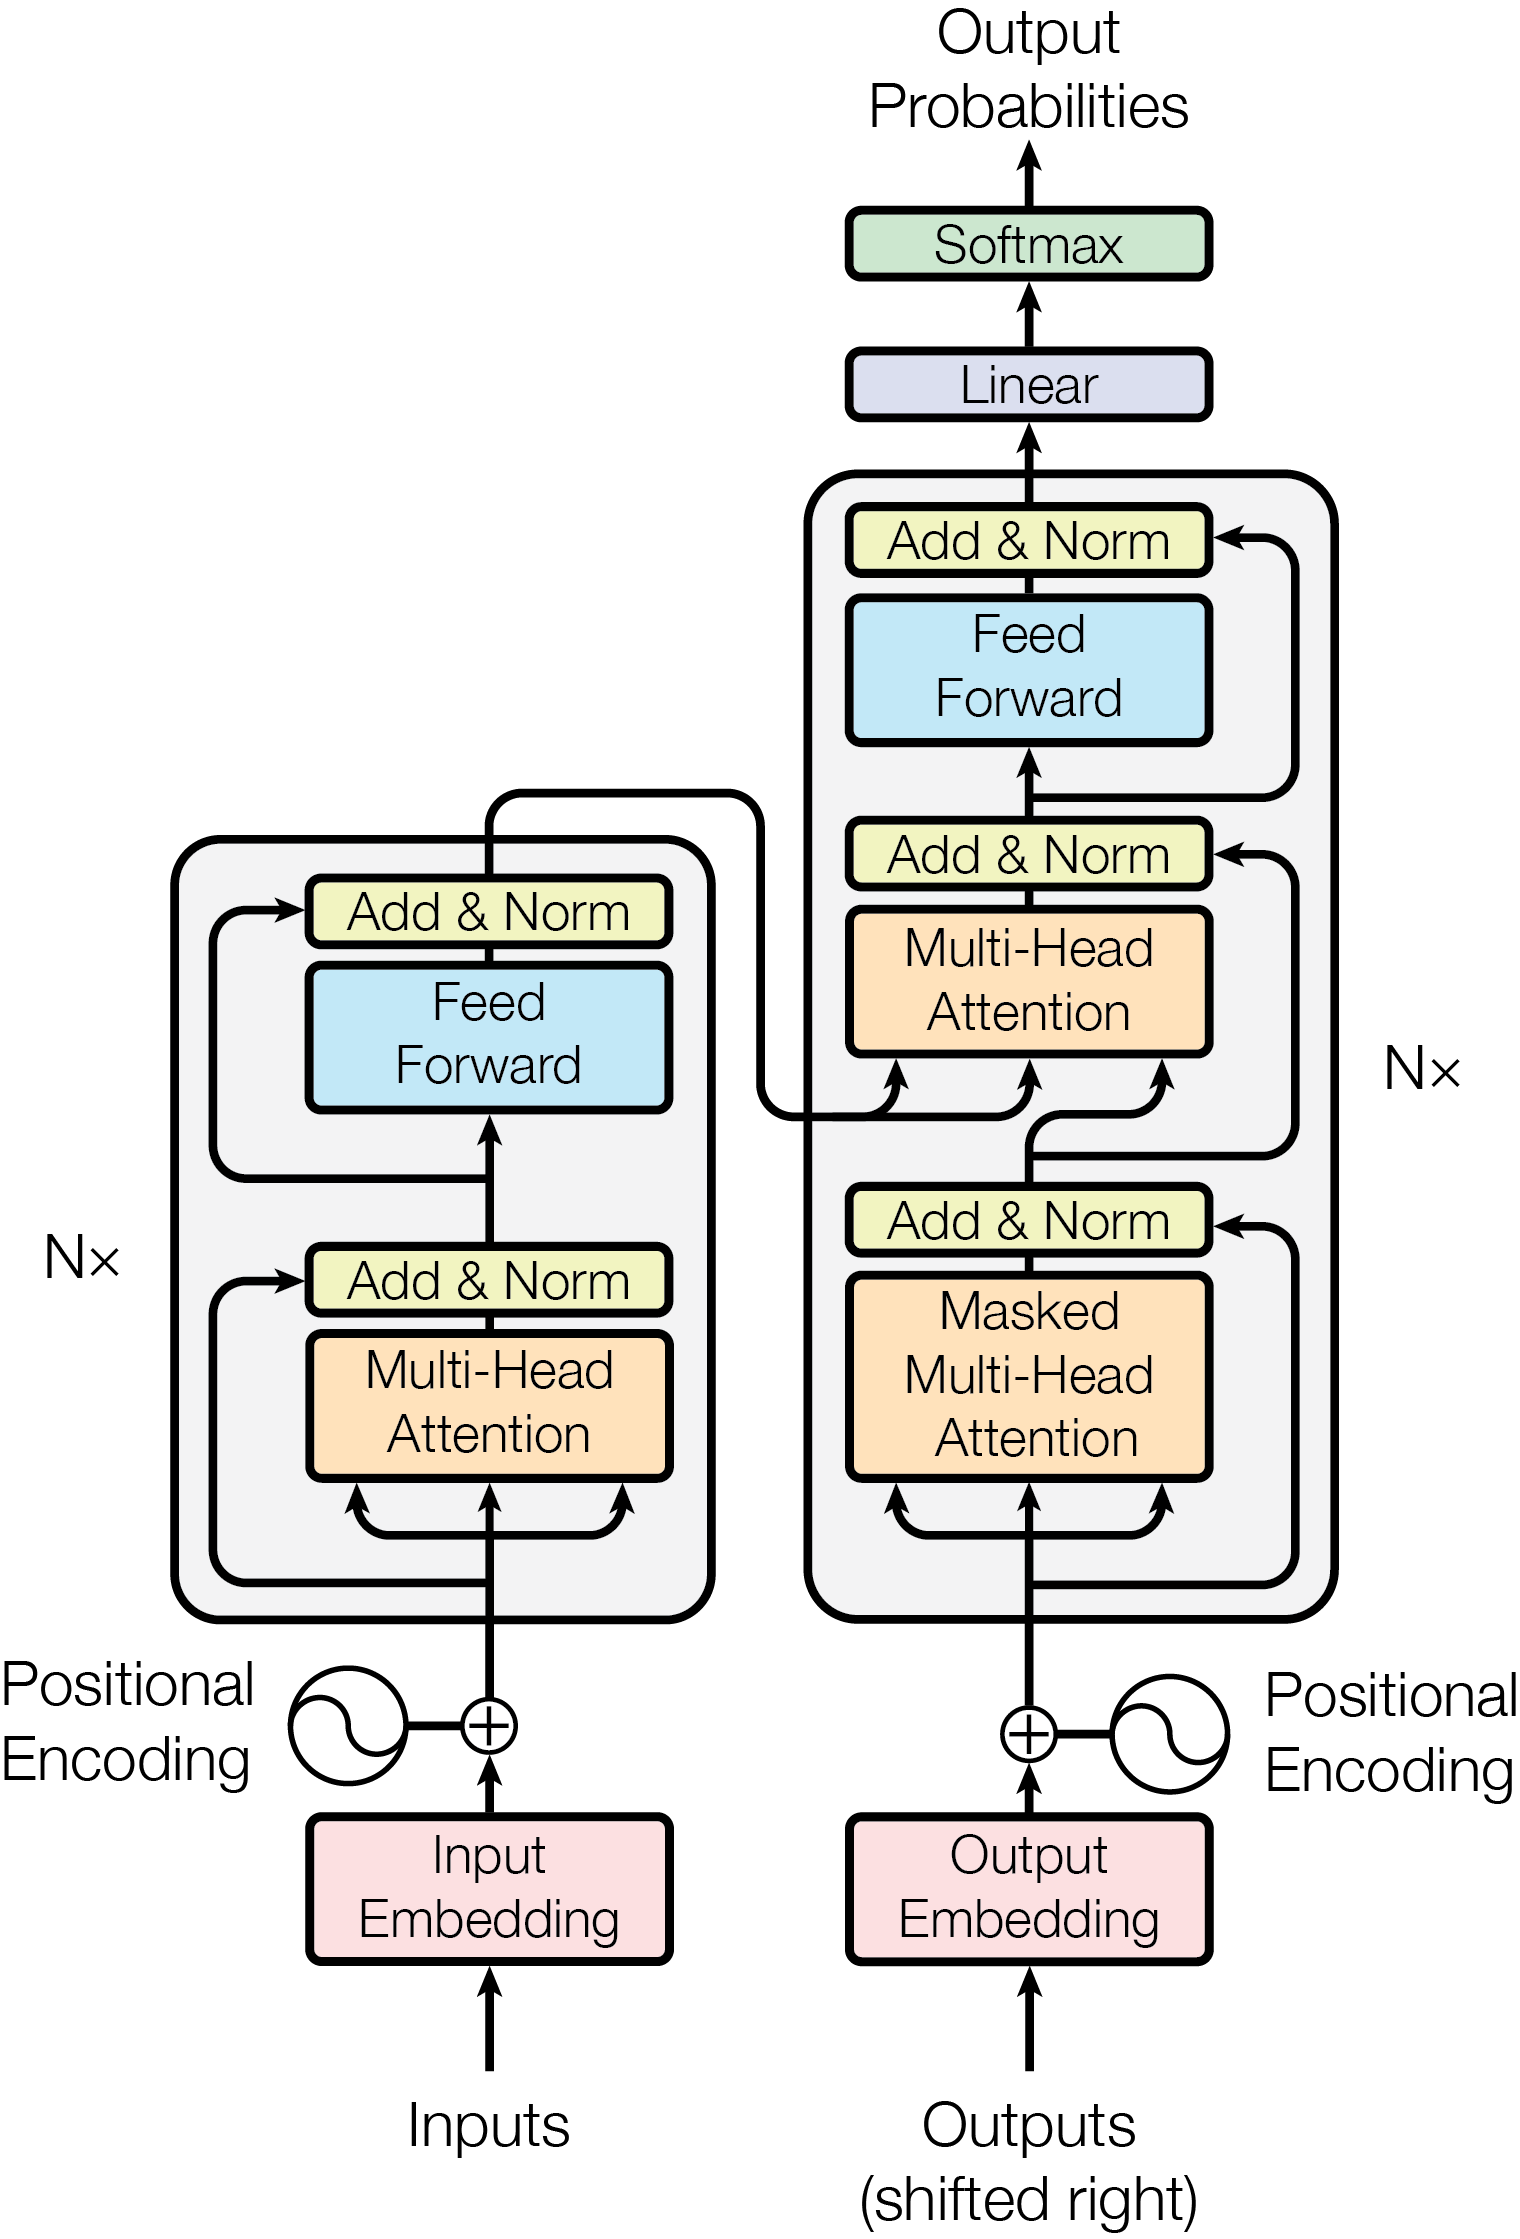
\includegraphics[width=0.6\linewidth]{example_images/transformer}
    \caption{The Transformer model architecture\cite{NIPS2017_3f5ee243}}
    \label{The Transformer model architecture}
  \end{figure}
\section{Dataset}